\section{Surface Parameterization Methods}
\label{sec:Surface-Parameterization-Methods}

This \cgal\ package implements some of the state-of-the-art
surface parameterization methods, such as Least Squares Conformal Maps,
Discrete Conformal Map, Discrete Authalic
Parameterization, Floater Mean Value Coordinates or Tutte Barycentric
Mapping. These methods are provided as models of the
\ccc{ParameterizerTraits_3} concept.


\subsection{Fixed Border Surface Parameterizations}

Fixed Border Surface Parameterizations need a set of constraints: two
(u,v) coordinates for each vertex along the border.
Such border parameterizations are described in Section
\ref{sec:Border-Parameterizations-for-Fixed-Methods}.

\subsubsection{Tutte Barycentric Mapping}

\ccc{CGAL::Barycentric_mapping_parameterizer_3<ParameterizationMesh_3, BorderParameterizer_3, SparseLinearAlgebraTraits_d>}  \\

The Barycentric Mapping parameterization method has been introduced by
Tutte~\cite{t-hdg-63}. In parameter space, each vertex is
placed at the barycenter of its neighbors to achieve the so-called
convex combination condition.

\emph{Complexity:}

This amounts to solve one
sparse linear solver for each set of parameter coordinates, with a
\#vertices x \#vertices sparse and symmetric positive definite matrix.
A coefficient $(i, j)$ of the matrix is set to 1 for an edge linking
the vertex $v_i$ to the vertex $v_j$, to minus the degree of the
vertex $v_i$ for a diagonal element, and to 0 for any other matrix
entry.

\emph{Guarantees:}

Always bijective when the border is convex.

\emph{Usage:}

Although Tutte Barycentric Mapping method is fast and
guaranteed to be bijective, it does not minimize angles nor areas
distortion.

% Insert image uniform.png/eps with
% title "Tutte Barycentric Mapping (the red line emphasizes the cutting path)"
\begin{center}
    \label{Surface_mesh_parameterization-fig-uniform}
    % Image
    \begin{ccTexOnly}
        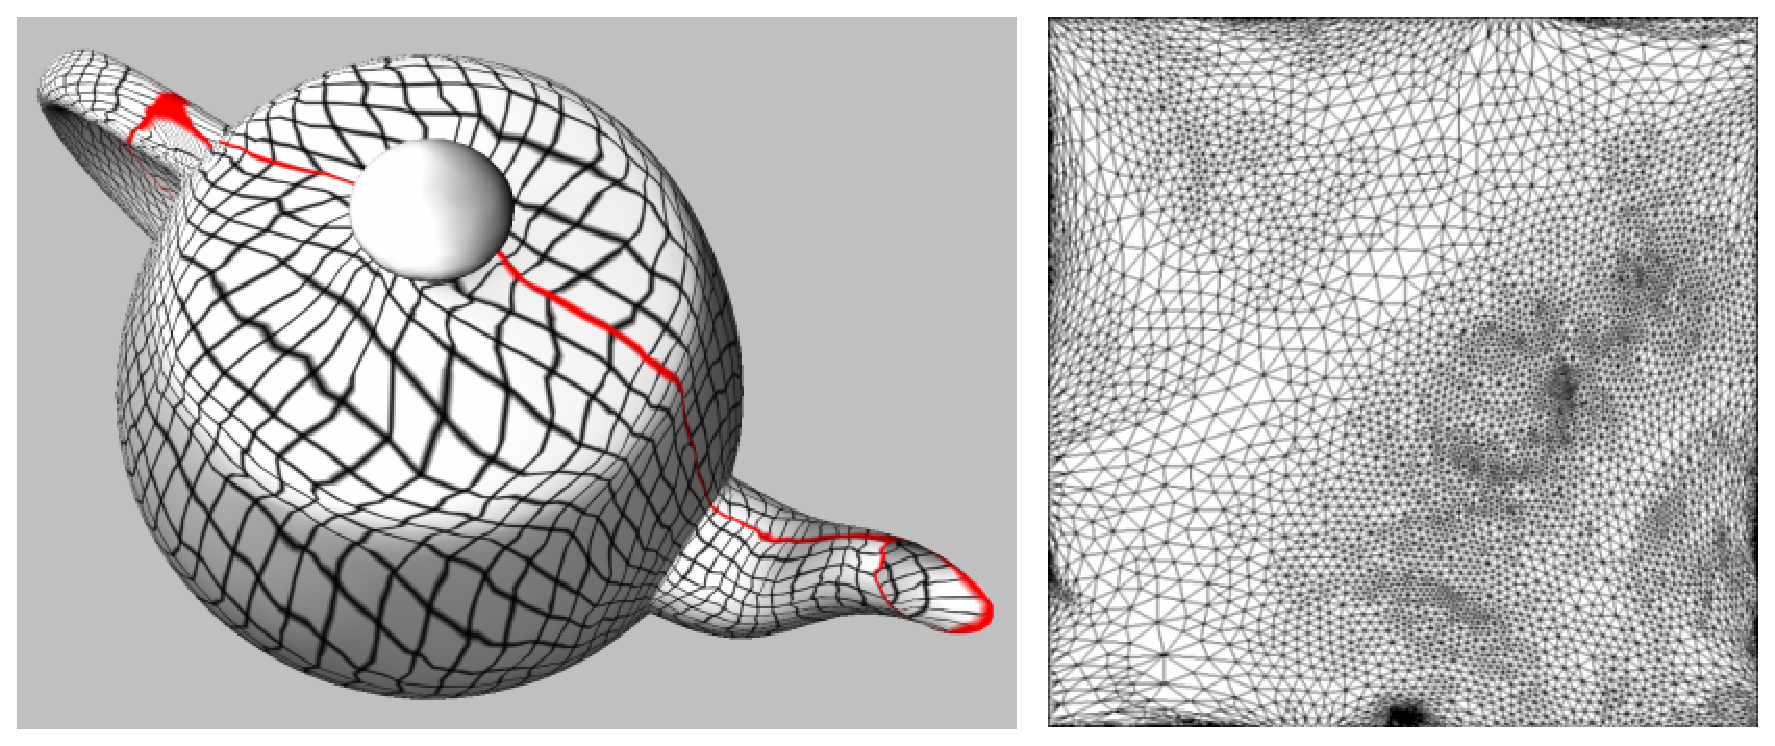
\includegraphics[width=0.45\textwidth]{Surface_mesh_parameterization/uniform}
    \end{ccTexOnly}
    \begin{ccHtmlOnly}
        <img width="45%" border=0 src="./uniform.png"><P>
    \end{ccHtmlOnly}
    % Title
    \begin{figure}[h]
        \caption{Tutte Barycentric Mapping (the red line emphasizes the cutting path)}
    \end{figure}
\end{center}

% Insert image uniform_2.png/eps with title "Teapot's image with Tutte Barycentric Mapping"
\begin{center}
    \label{Surface_mesh_parameterization-fig-uniform_2}
    % Image
    \begin{ccTexOnly}
        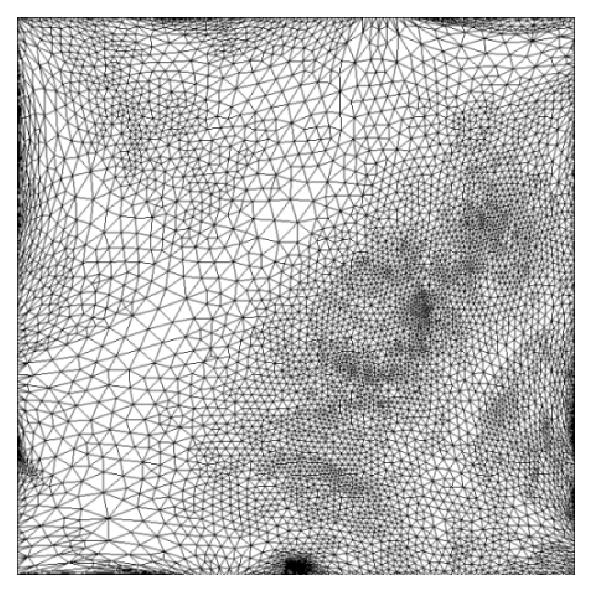
\includegraphics[width=0.45\textwidth]{Surface_mesh_parameterization/uniform_2}
    \end{ccTexOnly}
    \begin{ccHtmlOnly}
        <img width="45%" border=0 src="./uniform_2.png"><P>
    \end{ccHtmlOnly}
    % Title
    \begin{figure}[h]
        \caption{Teapot's image with Tutte Barycentric Mapping}
    \end{figure}
\end{center}


\subsubsection{Discrete Conformal Map}

\ccc{CGAL::Discrete_conformal_map_parameterizer_3<ParameterizationMesh_3, BorderParameterizer_3, SparseLinearAlgebraTraits_d>}  \\

Discrete Conformal Map parameterization has been introduced by Eck et
al. to the graphics community~\cite{cgal:eddhls-maam-95}.

\emph{Usage:}

It attempts to
lower angle deformation by minimizing a discrete version of the
Dirichlet energy as derived by Pinkall and
Polthier~\cite{cgal:pp-cdmsc-93}.
In practice, this gives visually nice results.

\emph{Guarantees:}

A one-to-one mapping is guaranteed only when two conditions are
fulfilled: the barycentric mapping condition (each vertex in parameter
space is a convex combination if its neighboring vertices) and the
border is convex.

% pierre: add cot figure, and detail what it means to have all weights
% positive, otherwise it is confusing.

\emph{Complexity:}

This method solves two \#vertices x \#vertices sparse linear
systems. The matrix (the same for both systems) is symmetric definite
positive, thus can be efficiently solved using dedicated linear
solvers.

% Insert image conformal.png/eps with title "Discrete Conformal Map"
\begin{center}
    \label{Surface_mesh_parameterization-fig-conformal}
    % Image
    \begin{ccTexOnly}
        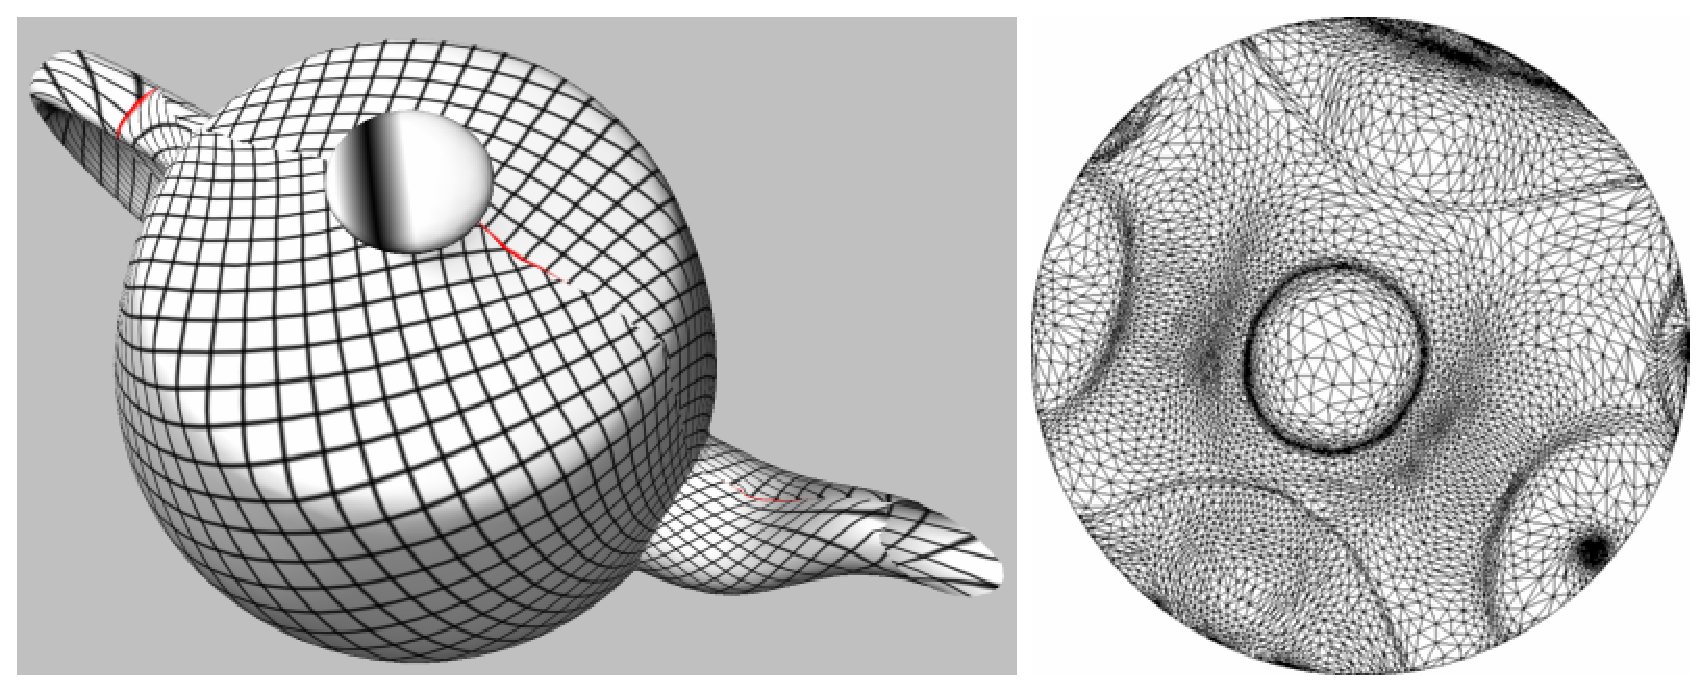
\includegraphics[width=0.45\textwidth]{Surface_mesh_parameterization/conformal}
    \end{ccTexOnly}
    \begin{ccHtmlOnly}
        <img width="45%" border=0 src="./conformal.png"><P>
    \end{ccHtmlOnly}
    % Title
    \begin{figure}[h]
        \caption{Discrete Conformal Map}
    \end{figure}
\end{center}

% Insert image conformal_2.png/eps with title "Teapot's image with Discrete Conformal Map"
\begin{center}
    \label{Surface_mesh_parameterization-fig-conformal_2}
    % Image
    \begin{ccTexOnly}
        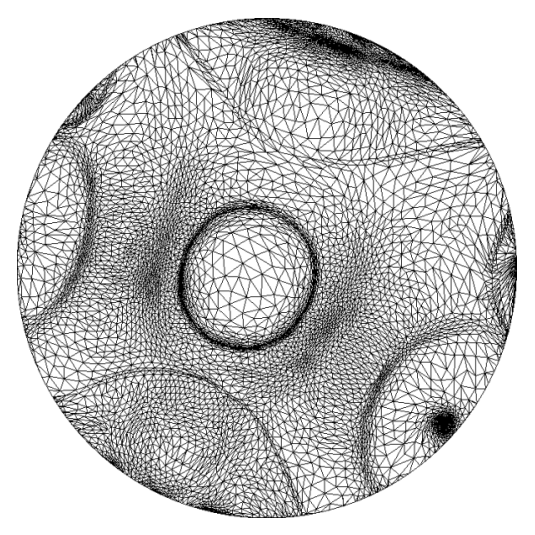
\includegraphics[width=0.45\textwidth]{Surface_mesh_parameterization/conformal_2}
    \end{ccTexOnly}
    \begin{ccHtmlOnly}
        <img width="45%" border=0 src="./conformal_2.png"><P>
    \end{ccHtmlOnly}
    % Title
    \begin{figure}[h]
        \caption{Teapot's image with Discrete Conformal Map}
    \end{figure}
\end{center}


\subsubsection{Floater Mean Value Coordinates}

\ccc{CGAL::Mean_value_coordinates_parameterizer_3<ParameterizationMesh_3, BorderParameterizer_3, SparseLinearAlgebraTraits_d>}  \\

The Mean Value Coordinates parameterization method has been introduced
by Floater~\cite{cgal:f-mvc-03}. Each vertex in parameter space is
optimized so as to be a convex combination of its neighboring
vertices. The barycentric coordinates are this time unconditionally
positive, by deriving an application of the mean theorem for harmonic
functions.

\emph{Usage:}

It is in essence an approximation of the Discrete Conformal
Maps, with a one-to-one mapping always guaranteed.

\emph{Guarantees:}

Always bijective when the border is convex.

\emph{Complexity:}

This method solves
two \#vertices x \#vertices sparse linear systems. The matrix (the
same for both systems) is asymmetric.

% Insert image floater.png/eps with title "Floater Mean Value Coordinates"
\begin{center}
    \label{Surface_mesh_parameterization-fig-floater}
    % Image
    \begin{ccTexOnly}
        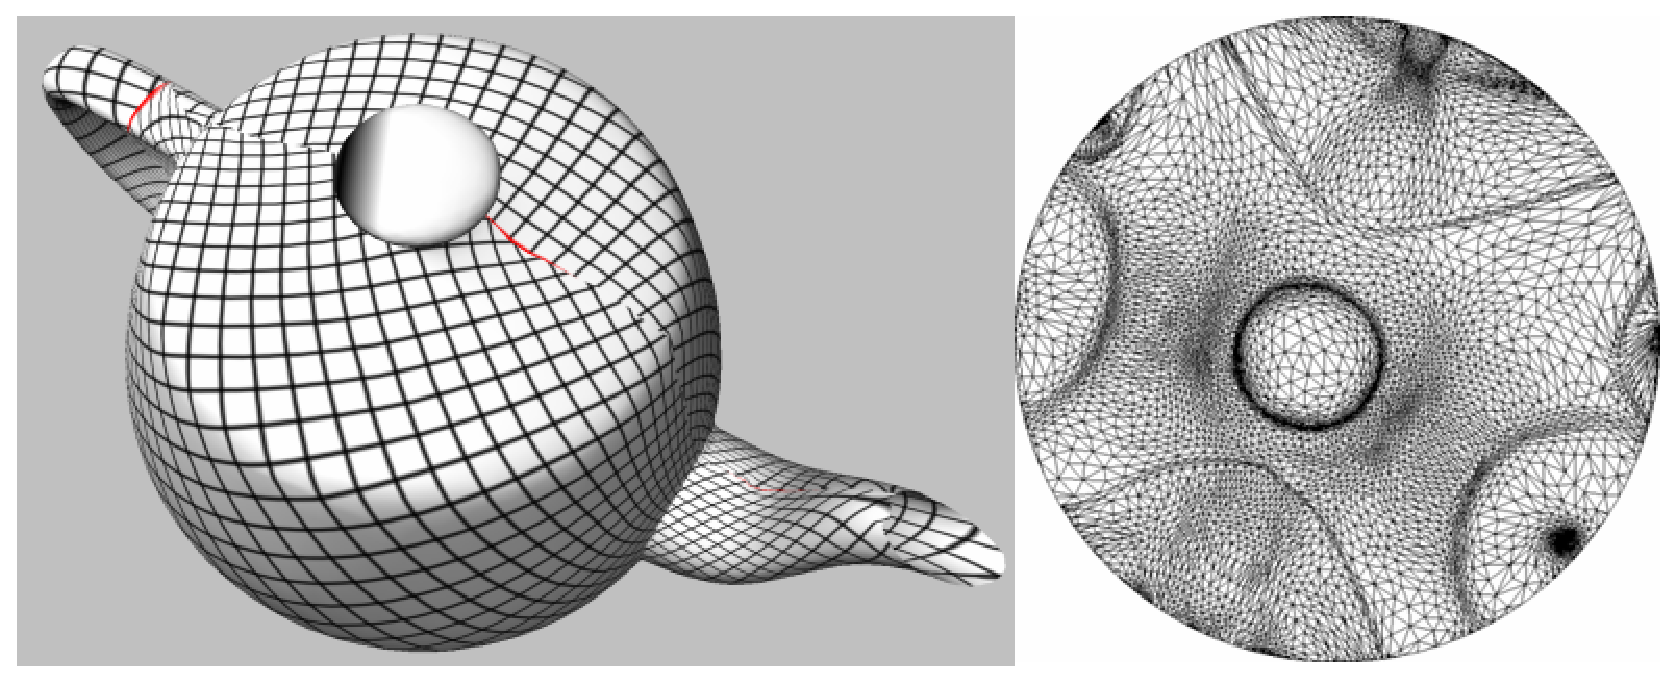
\includegraphics[width=0.45\textwidth]{Surface_mesh_parameterization/floater}
    \end{ccTexOnly}
    \begin{ccHtmlOnly}
        <img width="45%" border=0 src="./floater.png"><P>
    \end{ccHtmlOnly}
    % Title
    \begin{figure}[h]
        \caption{Floater Mean Value Coordinates}
    \end{figure}
\end{center}

% Insert image floater_2.png/eps with title "Teapot's image with Floater Mean Value Coordinates"
\begin{center}
    \label{Surface_mesh_parameterization-fig-floater_2}
    % Image
    \begin{ccTexOnly}
        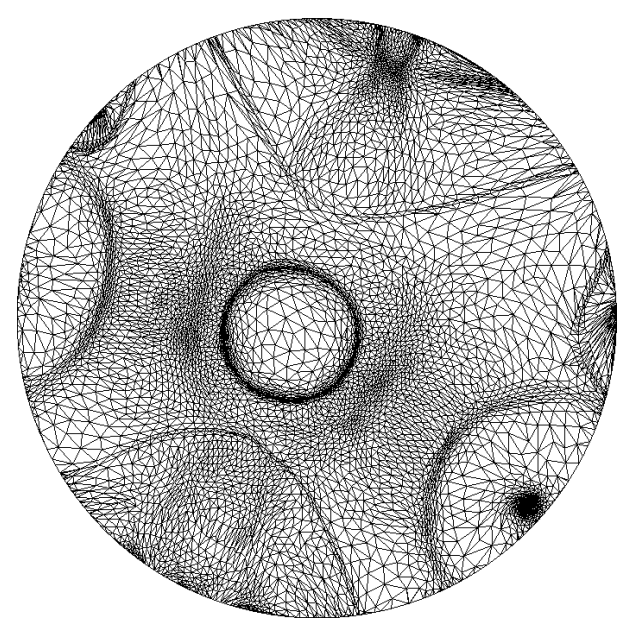
\includegraphics[width=0.45\textwidth]{Surface_mesh_parameterization/floater_2}
    \end{ccTexOnly}
    \begin{ccHtmlOnly}
        <img width="45%" border=0 src="./floater_2.png"><P>
    \end{ccHtmlOnly}
    % Title
    \begin{figure}[h]
        \caption{Teapot's image with Floater Mean Value Coordinates}
    \end{figure}
\end{center}


\subsubsection{Discrete Authalic parameterization}

\ccc{CGAL::Discrete_authalic_parameterizer_3<ParameterizationMesh_3, BorderParameterizer_3, SparseLinearAlgebraTraits_d>}  \\

The Discrete Authalic parameterization method has been introduced by
Desbrun, Meyer and Alliez~\cite{cgal:dma-ipsm-02}.

\emph{Usage:}

It corresponds to
a weak formulation of an area-preserving method, and in essence
locally minimizes the area distortion.

\emph{Guarantees:}

A one-to-one mapping is
guaranteed only if the convex combination condition is fulfilled and
the border is convex.

\emph{Complexity:}

 This method solves two
\#vertices x \#vertices sparse linear systems. The matrix (the same
for both systems) is asymmetric.

% Insert image authalic.png/eps with title "Discrete Authalic Parameterization"
\begin{center}
    \label{Surface_mesh_parameterization-fig-authalic}
    % Image
    \begin{ccTexOnly}
        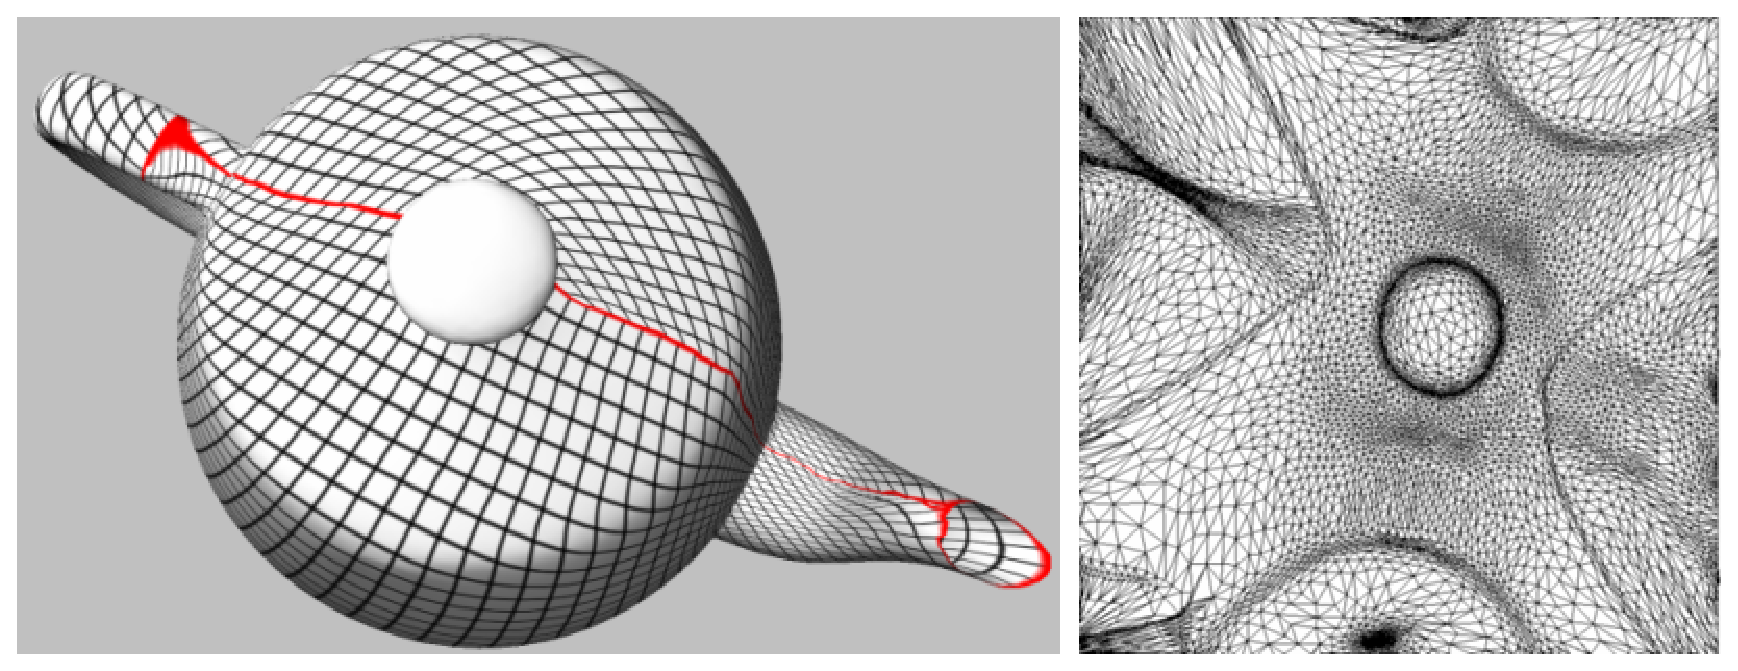
\includegraphics[width=0.45\textwidth]{Surface_mesh_parameterization/authalic}
    \end{ccTexOnly}
    \begin{ccHtmlOnly}
        <img width="45%" border=0 src="./authalic.png"><P>
    \end{ccHtmlOnly}
    % Title
    \begin{figure}[h]
        \caption{Discrete Authalic Parameterization}
    \end{figure}
\end{center}

% Insert image authalic_2.png/eps with title "Teapot's image with Discrete Authalic Parameterization"
\begin{center}
    \label{Surface_mesh_parameterization-fig-authalic_2}
    % Image
    \begin{ccTexOnly}
        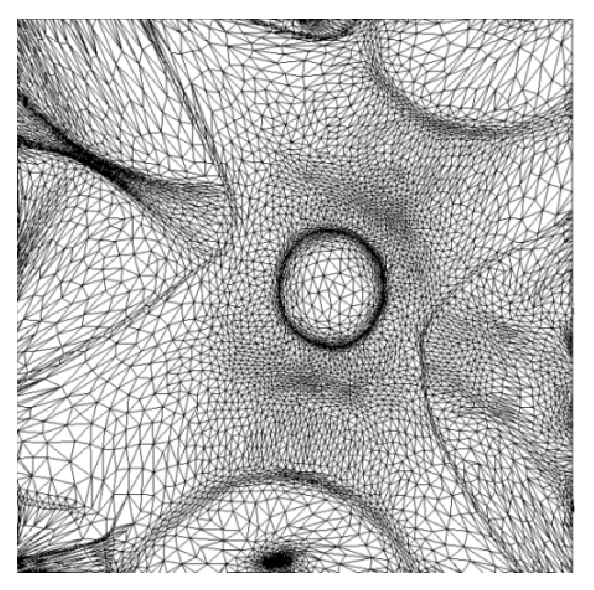
\includegraphics[width=0.45\textwidth]{Surface_mesh_parameterization/authalic_2}
    \end{ccTexOnly}
    \begin{ccHtmlOnly}
        <img width="45%" border=0 src="./authalic_2.png"><P>
    \end{ccHtmlOnly}
    % Title
    \begin{figure}[h]
        \caption{Teapot's image with Discrete Authalic Parameterization}
    \end{figure}
\end{center}


\subsubsection{Border Parameterizations for Fixed Methods}
\label{sec:Border-Parameterizations-for-Fixed-Methods}

Parameterization methods for
borders are used as traits classes modifying the behavior of
\ccc{ParameterizerTraits_3} models.
They are provided as models of the \ccc{BorderParameterizer_3} concept.

Border Parameterizations for Fixed Border Surface Parameterizations
are a family of methods to define a set of constraints, namely two
$u,v$ coordinates for each vertex along the border.

\begin{itemize}

\item
    The user can select a border parameterization among
    two commonly used methods: uniform or arc-length parameterization.

    \emph{Usage:}

    Uniform border parameterization is more stable, although it gives
    poor visual results. The
    arc-length border parameterization is used by default.

\item
    One convex shape specified by one shape among two standard ones:
    a circle or a square.

    \emph{Usage:}

    The circular border parameterization is used by default as it
    corresponds to the simplest convex shape. The square border
    parameterization is commonly used for texture mapping.

\end{itemize}

\ccc{CGAL::Circular_border_arc_length_parameterizer_3<ParameterizationMesh_3>}  \\
\ccc{CGAL::Circular_border_uniform_parameterizer_3<ParameterizationMesh_3>}  \\
\ccc{CGAL::Square_border_arc_length_parameterizer_3<ParameterizationMesh_3>}  \\
\ccc{CGAL::Square_border_uniform_parameterizer_3<ParameterizationMesh_3>}  \\

% Insert image circular_border.png/eps
% with title "Julius Cesar mask's image with Authalic/circular border"
\begin{center}
    \label{Surface_mesh_parameterization-fig-circular_border}
    % Image
    \begin{ccTexOnly}
        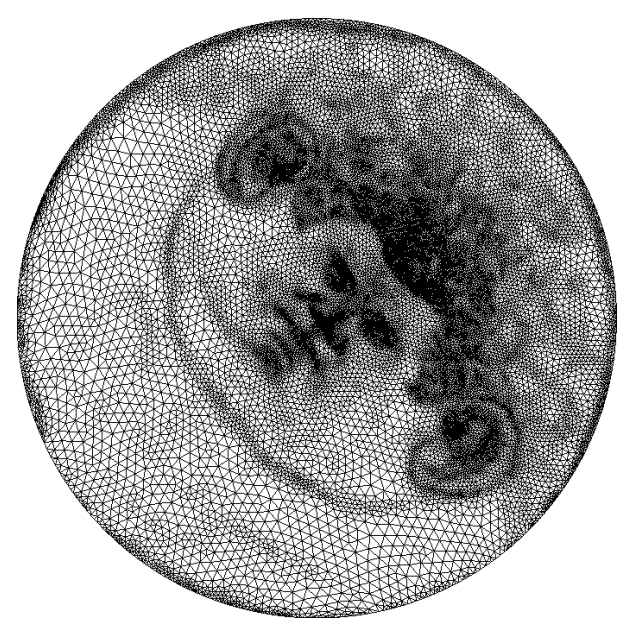
\includegraphics[width=0.35\textwidth]{Surface_mesh_parameterization/circular_border}
    \end{ccTexOnly}
    \begin{ccHtmlOnly}
        <img width="35%" border=0 src="./circular_border.png"><P>
    \end{ccHtmlOnly}
    % Title
    \begin{figure}[h]
        \caption{Julius Cesar mask's image with Authalic/circular border}
    \end{figure}
\end{center}

% Insert image square_border.png/eps
% with title "Julius Cesar mask's image with Floater/square border"
\begin{center}
    \label{Surface_mesh_parameterization-fig-square_border}
    % Image
    \begin{ccTexOnly}
        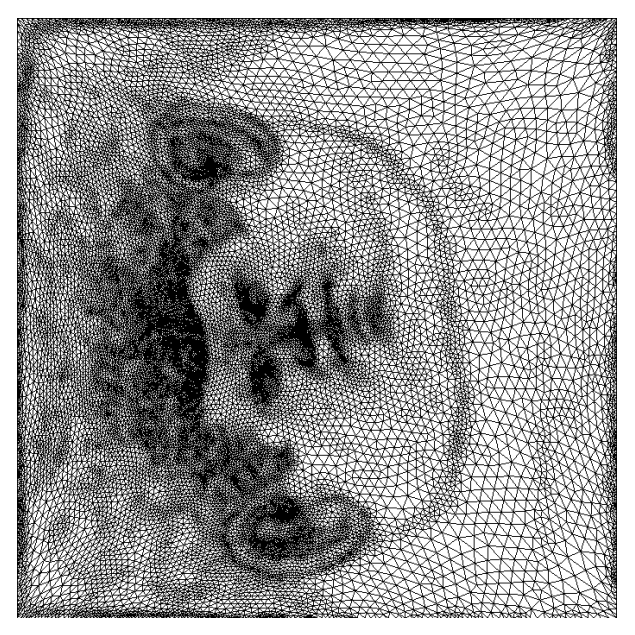
\includegraphics[width=0.35\textwidth]{Surface_mesh_parameterization/square_border}
    \end{ccTexOnly}
    \begin{ccHtmlOnly}
        <img width="35%" border=0 src="./square_border.png"><P>
    \end{ccHtmlOnly}
    % Title
    \begin{figure}[h]
        \caption{Julius Cesar mask's image with Floater/square border}
    \end{figure}
\end{center}


\subsection{Free Border Surface Parameterizations}

\subsubsection{Least Squares Conformal Maps}

\ccc{CGAL::LSCM_parameterizer_3<ParameterizationMesh_3, BorderParameterizer_3, SparseLinearAlgebraTraits_d>}  \\

The Least Squares Conformal Maps (LSCM) parameterization method has
been introduced by L\'evy et al.~\cite{cgal:lprm-lscm-02}.

\emph{Usage:}

It corresponds to a conformal method with a free border (at least two
vertices have to be constrained to obtain a unique solution), which
allows further lowering of the angle distortion.

\emph{Guarantees:}

A one-to-one mapping
is not guaranteed by this method.

\emph{Complexity:}

It solves a (2 $\times$
\#triangles) $\times$ \#vertices sparse linear system in the least squares sense,
which implies to solve a symmetric matrix.

% Insert image LSCM.png/eps with title "Least Squares Conformal Maps"
\begin{center}
    \label{Surface_mesh_parameterization-fig-LSCM}
    % Image
    \begin{ccTexOnly}
        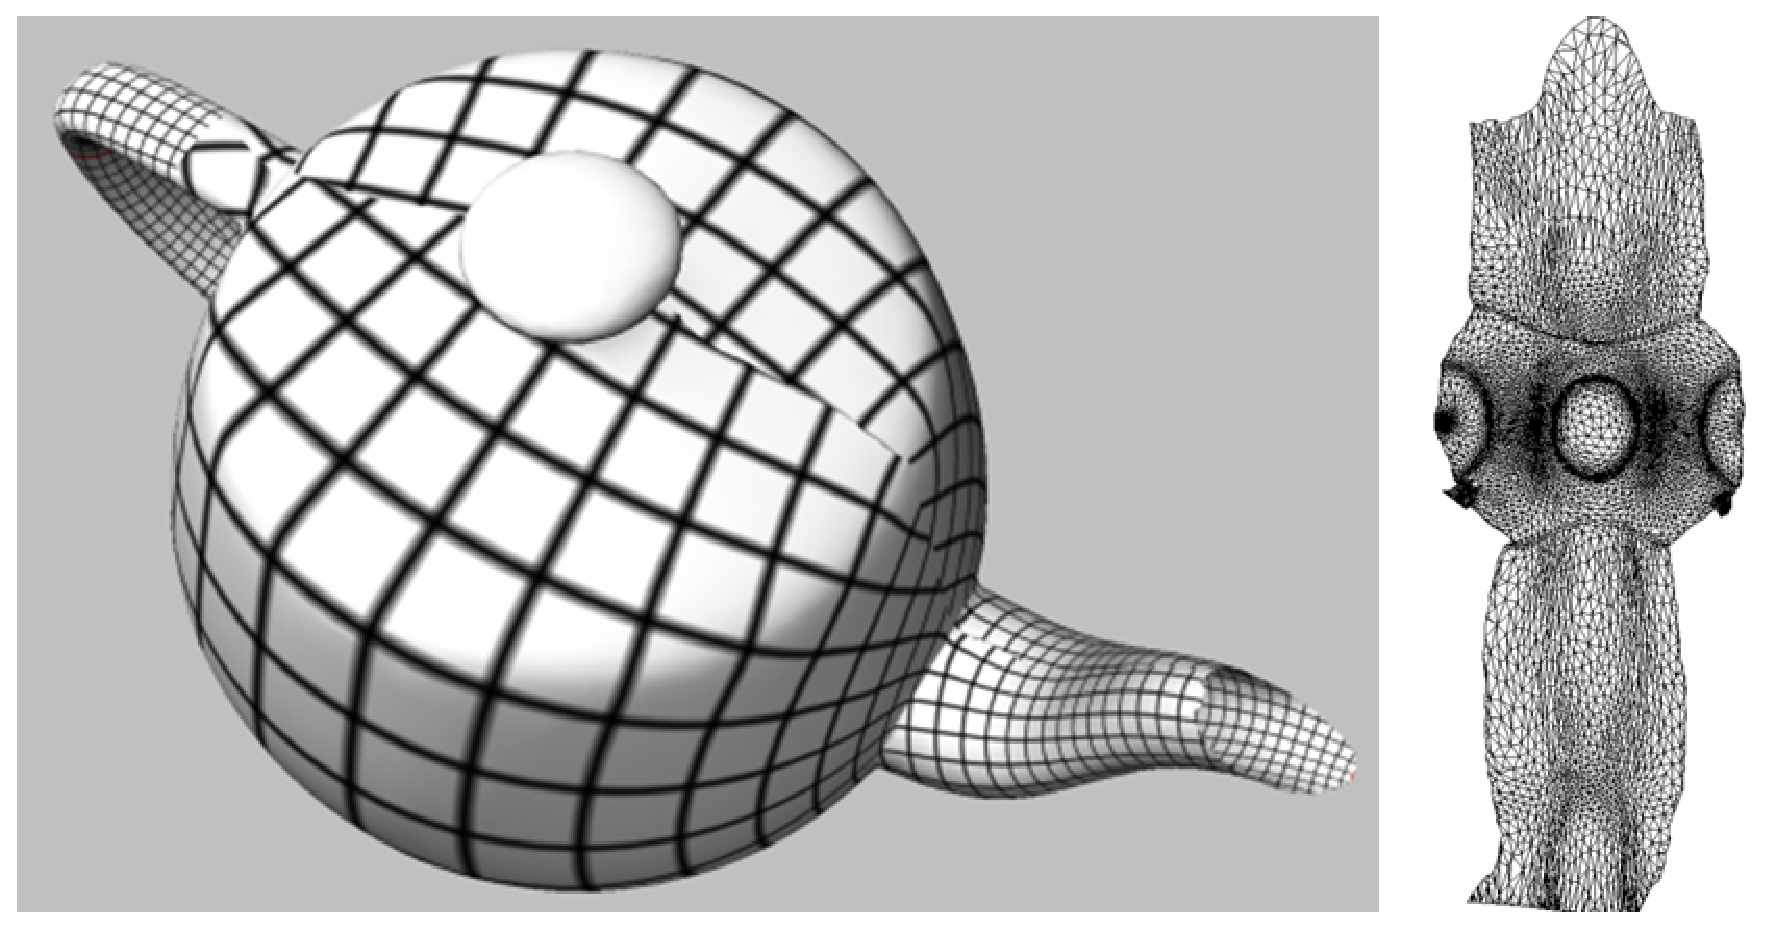
\includegraphics[width=0.45\textwidth]{Surface_mesh_parameterization/LSCM}
    \end{ccTexOnly}
    \begin{ccHtmlOnly}
        <img width="45%" border=0 src="./LSCM.png"><P>
    \end{ccHtmlOnly}
    % Title
    \begin{figure}[h]
        \caption{Least Squares Conformal Maps}
    \end{figure}
\end{center}

% Insert image LSCM_2.png/eps with title "Teapot's image with Least Squares Conformal Maps"
\begin{center}
    \label{Surface_mesh_parameterization-fig-LSCM_2}
    % Image
    \begin{ccTexOnly}
        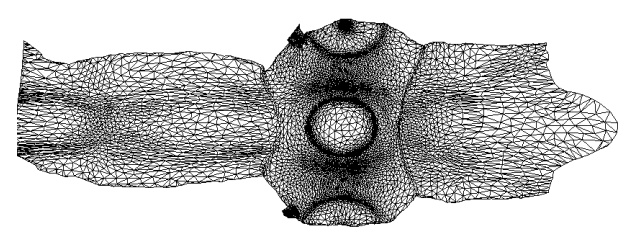
\includegraphics[width=0.75\textwidth]{Surface_mesh_parameterization/LSCM_2}
    \end{ccTexOnly}
    \begin{ccHtmlOnly}
        <img width="75%" border=0 src="./LSCM_2.png"><P>
    \end{ccHtmlOnly}
    % Title
    \begin{figure}[h]
        \caption{Teapot's image with Least Squares Conformal Maps}
    \end{figure}
\end{center}


\subsubsection{Border Parameterizations for Free Methods}
\label{sec:Border-Parameterizations-for-Free-Methods}

Parameterization methods for
borders are used as traits classes modifying the behavior of
\ccc{ParameterizerTraits_3} models.
They are provided as models of the \ccc{BorderParameterizer_3} concept.

The border parameterizations associated to Free Border Surface
Parameterization methods define only two constraints
(the pinned vertices).

\begin{itemize}

\item
    \ccc{CGAL::Two_vertices_parameterizer_3<ParameterizationMesh_3>}  \\

    \emph{Usage:}

    \ccc{CGAL::Two_vertices_parameterizer_3<ParameterizationMesh_3>} is the default
    free border parameterization (and in fact the only one available
    in the package today).

\end{itemize}


\subsection{Discrete Authalic Parameterization Example}

\ccc{Authalic_parameterization.C} computes a Discrete Authalic parameterization
over a \ccc{CGAL::Polyhedron_3<Traits>} mesh. Specifying a specific surface parameterization
instead of the default one means using the second parameter of \ccc{CGAL::parameterize()}.

The differences with the first example \ccc{Simple_parameterization.C} are:

\begin{ccExampleCode}

#include <CGAL/Discrete_authalic_parameterizer_3.h>

...

//***************************************
// Discrete Authalic Parameterization
//***************************************

typedef CGAL::Discrete_authalic_parameterizer_3<Parameterization_polyhedron_adaptor>
                                                    Parameterizer;

Parameterizer::Error_code err = CGAL::parameterize(mesh_adaptor, Parameterizer());

...

\end{ccExampleCode}


\subsection{Square Border Arc Length Parameterization Example}

\ccc{Square_border_parameterization.C} computes a Floater Mean Value Coordinates
parameterization with a Square Border Arc Length parameterization.
Specifying a specific border parameterization
instead of the default one means using the second parameter of
\ccc{CGAL::Mean_value_coordinates_parameterizer_3<ParameterizationMesh_3, BorderParameterizer_3, SparseLinearAlgebraTraits_d>}.

The differences with the first example \ccc{Simple_parameterization.C} are:

\begin{ccExampleCode}

#include <CGAL/Square_border_parameterizer_3.h>

...

//***************************************
// Floater Mean Value Coordinates parameterization
// with square border
//***************************************

// Square border parameterizer
typedef CGAL::Square_border_arc_length_parameterizer_3<Parameterization_polyhedron_adaptor>
                                                        Border_parameterizer;

// Floater Mean Value Coordinates parameterizer with square border
typedef CGAL::Mean_value_coordinates_parameterizer_3<Parameterization_polyhedron_adaptor,
                                                        Border_parameterizer>
                                                    Parameterizer;

Parameterizer::Error_code err = CGAL::parameterize(mesh_adaptor, Parameterizer());

...

\end{ccExampleCode}

